\section{Piecewise models as mixture models}
\label{sect:mix}

%%%%%%%%%%%%%%%%%%%%%%%%%
\begin{figure}
\centering
\begin{subfigure}{.48\linewidth}
\centering
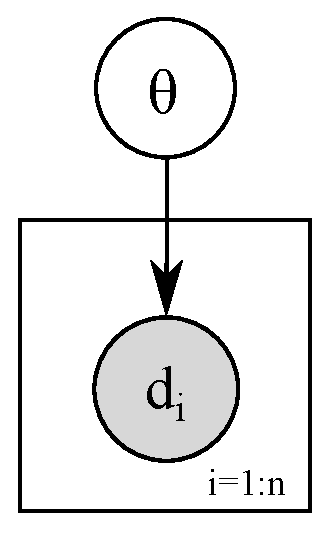
\includegraphics[width=.56\textwidth]{pic/naive.pdf}
\caption{}
\label{fig:naive}
\end{subfigure}
\begin{subfigure}{.48\linewidth}
\centering
  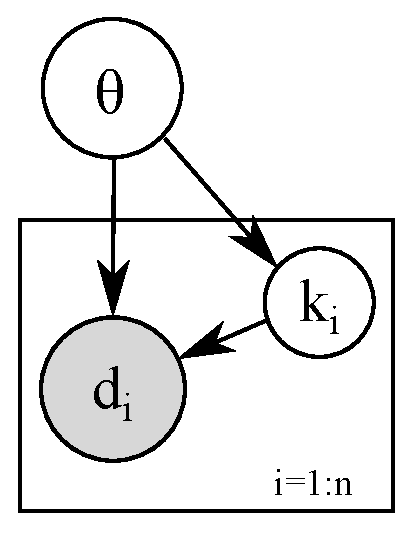
\includegraphics[width=.70\textwidth]{pic/naive-mix2.pdf}
\caption{}
\label{fig:naive.mix}
\end{subfigure}
\vspace{-2mm}
\caption{\footnotesize 
(a) A Bayesian inference model with parameter (vector) $\boldsymbol\theta$ and data points $d_1$ to $d_n$.
(b) A mixture model with parameter (vector) $\boldsymbol\theta$ and data points $d_1$ to $d_n$ 
}
\vspace{-5mm}
\end{figure}
%%%%%%%%%%%%%%%%%%%%%%%

%%%%%%%%%%%%%%%%%%%%%%%%%%%%%%%%%%%%%%
%We begin by considering Gibbs sampling on 
In this section we detail how to overcome the exponential complexity of standard Gibbs
sampling by transforming piecewise models to (augmented) mixture models and performing
linear time Gibbs sampling in this augmented model.  While augmented models to facilitate
Gibbs sampling have been proposed previously, e.g., Swendsen-Wang (SW) sampling~\cite{sw_mc} 
and more recently FlyMC sampling~\cite{fly_mc} methods like SW are specific to restricted
Ising models and FlyMC requires careful problem-specific proposal design and tuning.  In this paper,
we present a generic augmented model for an expressive class of piecewise models and
an analytical Gibbs sampler that does not require problem-specific proposal design.  
Furthermore, our Augmented Gibbs proposal achieves a novel \emph{exponential-to-linear reduction} in the complexity
of sampling from a Bayesian posterior with an exponential number of pieces.
%Furthermore, we achieve an \emph{exponential-to-linear reduction} in the computational complexity
%of sampling from a Bayesian posterior with an exponential number of pieces --- the first time
%we are aware such a result has been shown.

We motivate the algorithm by first introducing the augmented posterior for piecewise likelihoods:
\begin{align}
\label{e:expanded}
&pr(\boldsymbol\theta | \, d_1, \ldots, d_n) \, 
\propto 
pr(\boldsymbol\theta) \; \otimes
\\
&{\footnotesize
\begin{cases}
\boxed{k_1 = 1.} {\phi^{1}_{1}(\boldsymbol\theta)  : f^{1}_{1}(\boldsymbol\theta)}\\
\vdots
\\
\boxed{k_1 = M.} \phi^{1}_{M}(\boldsymbol\theta)  \!:\! f^{1}_{M}(\boldsymbol\theta)
\end{cases}
}%end font size
\!\!\!\!\!\!\!\!\!\!\!\!\!
\otimes
\cdots
\otimes
{\footnotesize
\begin{cases}
\boxed{k_n = 1.} \phi^{n}_{1}(\boldsymbol\theta)  : f^{n}_{1}(\boldsymbol\theta)\\
\vdots
\\
\boxed{k_n = M.} \phi^{n}_{M}(\boldsymbol\theta)  \!: f^{n}_{M}(\boldsymbol\theta)
\end{cases}
}%end font size
%\\= {\footnotesize
%\begin{cases}
%\phi_{1, 1}(\boldsymbol\theta) \wedge \ldots \wedge \phi_{n, 1}(\boldsymbol\theta) : f_{n, 1}(\boldsymbol\theta) \ldots f_{n, 1}(\boldsymbol\theta)\\
%\vdots
%\\
%\phi_{1, M}(\boldsymbol\theta) \! \wedge\! \ldots \!\wedge\! \phi_{n, M}(\boldsymbol\theta) \!:\! f_{n, 1}(\boldsymbol\theta) \ldots f_{n, M}(\boldsymbol\theta)
%\end{cases}
%}%end font size
\end{align} 
% It represents a Bayesian inference model in which likelihood functions are piecewise.
% Good point, but no space. -Scott
%
%\footnote{Clearly, prior distributions can be piecewise as well but since exponential blow up in the posterior structure is due to the amount of data, our focus is on likelihood functions.}
In the above, $k_i$ is the partition-counter of the $i$-th likelihood function. 
$\phi^i_{j}$ is its $j$-th constraint and
 $f^i_{j}$ is its associated sub-function. 
 Also for readability, case statements are numbered and without loss of
generality, we assume the number of partitions in each
likelihood function is $M$
%Remembering that $\phi^i_{1}$ to $\phi^i_{M}$ are mutually exhaustive and jointly exhaustive, 

We observe that each $k_i$ can be seen as a random variable. 
It deterministically takes the value of the partition whose associated constraint holds (given $\boldsymbol\theta$) and its possible outcomes are in $\textsc{Val}(k_i) = \{1, \ldots, M\}$. 
Note that for any given $\boldsymbol\theta$, exactly one constraint holds for a piecewise function, therefore, 
$\sum_{k_i = 1}^M pr(k_i \,|\, \boldsymbol\theta) = 1$.
Intuitively, it can be assumed that $k_i$ is the underlying variable that determines which partition of each likelihood function is `chosen'. As we have 
\begin{equation}
\label{e:aaaax}
pr(d_i | \, \boldsymbol\theta) = \sum_{k_i = 1}^M pr(k_i | \, \boldsymbol\theta) pr(d_i | \, k_i, \boldsymbol\theta) \text{,}
\end{equation}
we can claim that a piecewise likelihood function is a mixture model in which sub-function $f^i_j$ is the \emph{mixture component} and 
 $k_i$ provides binary \emph{mixture weight}. Hence:
%$$pr(d_i | \boldsymbol\theta) = \sum_{k_1}pr(k_1 | \, \boldsymbol\theta) pr(d_1 | \, k_1, \boldsymbol\theta)$$
%and
%\[pr(k_i = k \,|\, \theta) := {\footnotesize
%\begin{cases}
%\phi^i_k(\boldsymbol\theta)  &: 1\\
%\neg \phi^i_k(\boldsymbol\theta) &: 0
%\end{cases}
%}%end font size
%\]
%Provided with this definition, by Proposition~\ref{pro:discrete}, equation~(\ref{e:expanded}) can be restated as:
{\small
\begin{align*}
pr(\boldsymbol\theta | \, d_1, \ldots, d_n) 
&\propto
pr(\boldsymbol\theta) \otimes
\sum_{k_1}pr(k_1 | \, \boldsymbol\theta) pr(d_1 | \, k_1, \boldsymbol\theta) \\
&\qquad\qquad \otimes
\cdots \otimes
\sum_{k_n}pr(k_n | \, \boldsymbol\theta) pr(d_n | \, k_n, \boldsymbol\theta)
\\
&\propto
\sum_{k_1} \ldots \sum_{k_n} p(\boldsymbol\theta, d_1, \ldots, d_n, k_1, \ldots, k_n) 
\end{align*}}
This means that the Bayesian networks in Figures~\ref{fig:naive} and \ref{fig:naive.mix} are equivalent.
Therefore, instead of taking samples from \ref{fig:naive}, 
they can be taken from the \emph{augmented model} \ref{fig:naive.mix}. A key observation, however, is that 
unlike the conditional distributions $pr(\boldsymbol\theta_i | \, \boldsymbol\theta_{-i})$, 
in $pr(\boldsymbol\theta_i | \boldsymbol\theta_{-i}, k_1, \ldots, k_n)$ 
the number of partitions is constant rather than growing as $M^n$.
% ---
%yielding the desired \emph{exponential-to-linear} reduction.
% in the time to compute 
%$pr(\boldsymbol\theta_i | \boldsymbol\theta_{-i}, k_1, \ldots, k_n)$ that forms
%the first key insight of the paper.
%
%As an instance, for $n=2$,   $k_1 = M$ and $k_2 = 1$:

The reason is that if  $\bvec{k}=k_1, \ldots, k_n$ are given, for $i$-th 
likelihood, a single sub-function $f^i_{k_i}$ is `chosen' and
$pr(\boldsymbol\theta_i | \boldsymbol\theta_{-i}, k_1, \ldots, k_n) = 
pr(\boldsymbol\theta | \boldsymbol\theta_{-i})\prod_{k_i} f^i_{k_i}(\boldsymbol\theta_i | \boldsymbol\theta_{-i})$.
Since the sub-functions are not piecewise themselves, 
the number of partitions in $pr(\boldsymbol\theta_i | \boldsymbol\theta_{-i},  k_1, \ldots, k_n)$ is bound by the number of partitions in the prior.

In the following proposition, we prove Equation~(\ref{e:aaaax}) is valid:
%\[
%p(x_i |\, \bvec{x}_{i-1}, \bvec{k}) = 
 % f_{1, 2}(\bvec{x}) \ldots f_{n, 2}(\bvec{x})
%\]  
\begin{comment}
\begin{equation}
\label{e:dodo}
pr\left(
{\footnotesize
\begin{cases}
{\phi^{1}_{1}(\boldsymbol\theta)  : f^{1}_{1}(\boldsymbol\theta)}\\
\vdots
\\
\boxed{\phi^{1}_{M}(\boldsymbol\theta)  : f^{1}_{M}(\boldsymbol\theta)}
\end{cases}
}
\otimes 
{\footnotesize
\begin{cases}
\boxed{\phi^{2}_{1}(\boldsymbol\theta)  : f^{2}_{1}(\boldsymbol\theta)}\\
\vdots
\\
\phi^{2}_{M}(\boldsymbol\theta)  :  f^{2}_{M}(\boldsymbol\theta)
\end{cases}
}
, k_1 = M, k_2 = 1\right)
= f^{1}_{M}(\boldsymbol\theta)  f^{2}_{1}(\boldsymbol\theta)
%end font size
\end{equation}


\section{Piecewise models as mixture models}
\label{sect:mix}

Consider a piecewise likelihood function in equation~(\ref{e:piecewise.likelihood22}). 
A simple but key observation is that since the constraints, $\phi_j$, exhaustively partition the space of $\boldsymbol \theta$,
we can define an \emph{auxiliary} (or \emph{augmented}) random variable $k$ with $M$ possible outcomes, $\text{Val} (k) := \{1, \, \ldots, \, M\}$,
such that 
$pr(k = i |\, \boldsymbol\theta) = 1$ if and only if $\phi_i (\boldsymbol\theta) = \top$. %\footnote{Note that $\sum_{k_i} pr (k_i | \, \boldsymbol \theta) = 1$.}%end footnote. 
As the following shows,
a piecewise model can be reinterpreted as a \emph{mixture model} 
which is the result of marginalizing over the \emph{intermediate} random variables $k$.
This means that graphical models depicted in Figures~\ref{fig:naive} and \ref{fig:naive.mix} are equivalent.
\end{comment}
%----------------------------------------***
\begin{proposition}
\label{pro:discrete}
The piecewise likelihood function $pr(d | \, \boldsymbol\theta)$ 
defined by (\ref{e:piecewise.likelihood22}) is equivalent to 
$\sum_{k = 1}^M pr(k | \, \boldsymbol\theta) pr(d | \, k, \boldsymbol\theta)$
where:
%\noindent\begin{minipage}{.5\linewidth}
%\begin{align}
{\footnotesize
\begin{eqnarray}
pr(d | \, \boldsymbol\theta) &:=& 
\begin{cases}
\phi^d_1(\boldsymbol\theta)  &: f^d_1(\boldsymbol\theta)\\
									  &\vdots\\
\phi^d_M(\boldsymbol\theta)  &: f^d_M(\boldsymbol\theta)
\end{cases}
\label{e:piecewise.likelihood22}
\\
%end font size 
% \end{equation}
%\end{minipage}%
%\begin{minipage}{.5\linewidth}
% \begin{equation}
pr(k |\, \boldsymbol\theta) &:=& 
\begin{cases}
\phi_k(\boldsymbol\theta)  &: 1\\
\neg \phi_k(\boldsymbol\theta) &: 0
\end{cases}
\label{e:2rel22}
\\
%end font size
% \end{equation}
% \begin{equation}
pr(d | \, k, \boldsymbol\theta) &:=& f^d_k(\boldsymbol\theta)
\label{e:2rel222}
\end{eqnarray}
}
%\end{align}
%\end{minipage}
%
\end{proposition}


\begin{proof}
Since constraints $\phi_k$ are mutually exclusive and jointly exhaustive: 
$$\sum_{k= 1}^N pr(k | \, \boldsymbol\theta) = 
\sum_{k=1}^N
{\footnotesize
\begin{cases}
\phi_k(\boldsymbol\theta)   &: 1\\
\neg \phi_k(\boldsymbol\theta)  &: 0
\end{cases}
}%end font size
\, =1
$$
Therefore $pr(k | \, \boldsymbol\theta)$ is a proper probability function. 
On the other hand, by marginalizing $k$, (\ref{e:2rel22}) and (\ref{e:2rel222}) trivially lead to (\ref{e:piecewise.likelihood22}):
{\small 
\begin{align*}
\sum_{k} pr(k | \, \boldsymbol\theta)pr(d | \, k, \boldsymbol\theta) 
&= 
\sum_{k=1}^N  
{\footnotesize
\begin{cases}
\phi_k(\boldsymbol\theta)  &: 1\\
\neg \phi_k(\boldsymbol\theta) &: 0
\end{cases}
}%end font size
\, \cdot \, f^d_k(\boldsymbol \theta)
&&\text{\hspace{-5mm}by (\ref{e:2rel22}), (\ref{e:2rel222})}
\\
&=
\sum_{k=1}^N 
{\footnotesize
\begin{cases}
		\phi_k(\boldsymbol\theta)  &: f^d_k(\boldsymbol\theta)\\
\neg 	\phi_k(\boldsymbol\theta)  &: 0
\end{cases}
}%end font size
\nonumber \\
&= {\footnotesize
\begin{cases}
\phi_1(\boldsymbol\theta)  &: f^d_1(\boldsymbol\theta)\\
\vdots\\
\phi_n(\boldsymbol\theta)  &: f^d_N(\boldsymbol\theta)
\end{cases}
}%end font size
= pr(d | \, \boldsymbol\theta) 
&&\text{\hspace{-2mm}by (\ref{e:piecewise.likelihood22})}
\end{align*}}
in which the third equality holds since constraints $\phi_k$ are mutually exclusive. 
\end{proof}
%Proposition~\ref{pro:discrete} shows that a piecewise model can be augmented to an equivalent model  via augmenting it with auxiliary random variables. The difference is that the order of complexity of Gibbs sampling on the latter model is significantly lower.However, two subtle problems are remained that will be addressed in the next subsections. %as the next subsection shows, it causes a \emph{deterministic dependencies problem} that should be addressed first.
 
\subsection{Deterministic dependencies and blocked sampling}
\label{sect:deterministic}
%%%%%%%%%%%%%%%%%%%%%%%%%
\begin{figure}
  \centering
  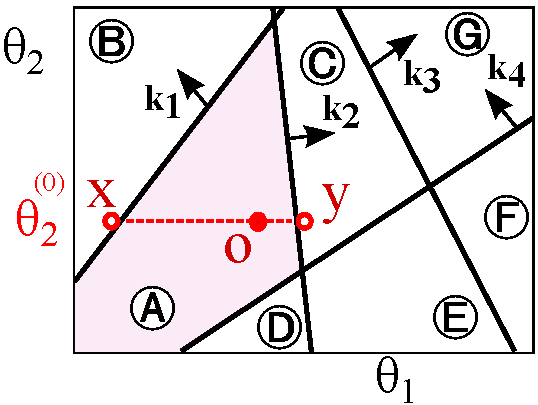
\includegraphics[width=0.25\textwidth]{pic/colxx.pdf}
\caption{\footnotesize
A piecewise joint distribution of $(\theta_1, \theta_2)$ partitioned by bi-valued linear constraints.
% with associated auxiliary variables $k_i$.
In the side, specified by each arrow, its associated auxiliary variable $k_i$ is 1 otherwise 2.
A Gibbs sampler started from an initial point $O = (\theta_1^{(0)}, \theta_2^{(0)})$, is trapped in an initial partition (A) 
where $k_1 = k_2 = k_3 = 1$ and $k_4 = 2$. 
}
\label{fig:simple.example}
\end{figure}
%%%%%%%%%%%%%%%%%%%%%%%
\paradot{Deterministic dependencies} It is known that in the presence of determinism Gibbs sampling gives poor results \cite{Poon:06}.
In our setting, deterministic dependencies arise from Definition~(\ref{e:2rel22}), were the value of $k$ is  decided by $\boldsymbol{\theta}$.
This problem is illustrated in Figure~\ref{fig:simple.example} by a simple example:
A Gibbs sampler started from an initial point $O=(\theta_1^{(0)}, \theta_2^{(0)})$, 
is trapped in the initial partition (A). 
The reason is that conditioned on the initial value of the auxiliary variables, 
the partition is deterministically decided as being (A), and conditioned on any 
point in (A), the auxiliary variables kept their initial values. %I.e.\ only on 
%line segment $xy$, $pr(\theta_1 | \theta_2^{(0)}, k_1^{(0)}, \ldots, 
%k_4^{(0)}) 
%>0$, etc.

%To illustrate the problem that emerges by Gibbs sampling on the mixture model defined by Proposition~\ref{pro:discrete}, consider the simple piecewise model depicted in Fig.~\ref{fig:simple.example} on a 2D parameter space $\boldsymbol\theta = (\theta_1, \theta_2)$ with a 2-piece prior, two observed points with a 2-piece and a 3-piece corresponding likelihood models. We augment the model by introducing auxiliary random variables $\bvec{k} = \{k_1, k_2\}$ such that $\textsc{Val}(k_1) = \{1,2,3\}$ and $\textsc{Val}(k_2) = \{1,2\}$ indicating (the constrain of) which partition in each likelihood function holds. Suppose Gibbs sampling is executed on the augmented model, starting from an initial point $(\theta_1^{(0)}, \theta_2^{(0)}, k_1^{(0)} = 2, k_2^{(0)} = 1)$ (shown in Fig~\ref{fig:blocking}a as a filled red circle). Firstly, $\theta$ is conditionally sampled: $\theta_1^{(1)} \sim pr(\theta_1 | \, \theta_2^{(0)}, k_1^{(0)}, k_2^{(0)}) $ In Fig~\ref{fig:blocking}a, the interval on which this conditional distribution is non-zero is depicted with a red dashed line segment. Clearly $\theta_1^{(1)}$ will be located inside partition (A) or (B) where $k_1 = 2$ and $k_2 = 1$ (i.e.\ second constraint of the first likelihood and the first constraint of the second likelihood function hold). In the second step, $\theta_2$ is sampled (see Fig.~\ref{fig:blocking}b): $\theta_2^{(1)} \sim pr(\theta_2 | \, \theta_1^{(1)}, k_1^{(0)}, k_2^{(0)})$ which again lies in either (A) or (B). In the next step  $k_1^{(1)} \sim pr(k_1 | \, \theta_1^{(1)}, \theta_2^{(1)}, k_2^{(0)})$ would deterministically take its former value $k_1^{(0)}$ since it is decided by $\boldsymbol\theta^{(1)}$. Similarly, $k_2^{(1)} = k_2^{(0)}$. By following this process, it can clearly be seen that all generated particle(s) will remain in the union of partitions (A) and (B).  This example reveals that Gibbs sampling on an augmented model is trapped in an initial set of partitions that specify the initial value of auxiliary variables). A way round this problem is provided in the next subsection.  
%%%%%%%%%%%%%%%%%%%%%%%%%%%%%%
%\subsection{Blocked Gibbs sampling on mixture models}
%\label{sect:collapsed}
%%
%%%%%%%%%%%%%%%%%%%%%%%%%%%%%%%%%%%%%%%%%%%%%%%%%%%%%%%%%%%%%%%%%%%%%%%%%%%%%%%%%%%%%%%%%%%
%% NOTE TO HADI: need to define the sampler!  Symbolic CDF then binary search for inverse!
%%               also need to clean up conditioning on data; also partition for datum d?
%%%%%%%%%%%%%%%%%%%%%%%%%%%%%%%%%%%%%%%%%%%%%%%%%%%%%%%%%%%%%%%%%%%%%%%%%%%%%%%%%%%%%%%%%%%
%%
\paradot{Blocked Gibbs}
We avoid deterministic dependencies by Blocked sampling:
at each step of Gibbs sampling, a parameter variable $\boldsymbol\theta_i$ is 
jointly sampled with  
(at least) one auxiliary variable $k_j$ 
conditioned on the remaining variables:
$
(\boldsymbol\theta_i, k_j) \sim pr(\boldsymbol\theta_i, k_j | \, \boldsymbol 
\theta_{-i}, 
\bvec{k}_{-j})  
$.
%(\emph{blocked Gibbs sampling}).
Since 
$pr(\boldsymbol\theta_i, k_j | \, \boldsymbol \theta_{-i}, \bvec{k}_{-j}) = 
pr(\boldsymbol\theta_i | \, \boldsymbol \theta_{-i}, \bvec{k}_{-j})\cdot pr(k_j 
| \, \boldsymbol\theta)$,  
this is done in 2 steps:
\begin{enumerate}
\item 
$k_j$ is marginalized out and $\boldsymbol\theta_i$ is sampled (\emph{collapsed 
Gibbs sampling}):
$$
\boldsymbol\theta_i \sim \sum_{k_j} 
pr(k_j | \, \boldsymbol \theta_{-i}, \bvec{k}_{-j}) 
pr(\theta_i | \, k_j, \boldsymbol \theta_{-i}, \bvec{k}_{-j})  
$$
\item
$k_j$ is determined from $\boldsymbol \theta$:
$k_j \leftarrow i \in \textsc{Val}(k_j)$ s.t.\ $\phi_i^j(\boldsymbol \theta) = \textit{true}$
where $\phi_i^j$ is the $i$-th constraint of $j$-th likelihood function.
\end{enumerate}

For instance in Figure~\ref{fig:simple.example}, for sampling $\theta_2$, 
either $k_1$ or $k_2$ is collapsed,
then the next sample will be in the union of partition (A) with either (B) or (C). 

%This trick is illustrated in Fig.~(\ref{fig:blocking}c) where $(\theta_1, k_2)$ are sampled jointly, followed by joint sampling of $(\theta_2, k_1)$ in (in Fig.~\ref{fig:blocking}d). 
%Using this method, (at least for some combinations of auxiliary and parameter variables) deterministic dependencies does not occur. This prevents being trapped in a single subset of partitions.
\paradot{Targeted selection of collapsed auxiliary variables}
We provide a mechanism for finding auxiliary variables $k_j$ that, with a high  
probability, are not determined by the other auxiliary variables, 
$\bvec{k}_{-j}$ when jointly sampled with a parameter variable 
$\boldsymbol\theta_i$. 
We observe that the set of partitions satisfying the current valuation of $\bvec{k}$
often differs with its adjacent partitions in a single auxiliary variable.
Since such a variable is not determined by other variables, it can be used in 
the blocked sampling.

However, in case some likelihood functions share the same constraint, some 
adjacent partitions would differ in multiple auxiliary variables.
In such cases, more than one auxiliary variable should be used in blocked sampling.

Finding such auxiliary variables has a simple geometric interpretation. As 
such, we explain it by a simple 
example depicted in Figure~(\ref{fig:simple.example}).
Consider finding a proper $k_j$ 
for blocked sampling $pr(\boldsymbol\theta_1, k_j | \, 
\boldsymbol\theta_2^{(0)}, \bvec{k}_{-j})$. 
It suffices to extend the line segment $pr(\boldsymbol\theta_1 | \, 
\boldsymbol\theta_2^{(0)}, \bvec{k})>0$ in two sides to reach the point $x$ or 
$y$. In this way, the neighboring partition e.g.\ (B) and (C) and consequently 
their corresponding $\bvec{k}$ valuations are detected. 
Finally, the auxiliary variables that differ between (A) and (B) or differ between (A) and (C)) are found ($k_1$ and $k_2$, in the Figure~(\ref{fig:simple.example})). 
%Clearly by block sampling these variables with $\theta_1$, deterministic dependency problem is avoided.
%By comparing the auxiliary variables that differs between (C) and the union of (A) \& (B) which is $k_2$. This is exactly how, blocked sampling is carried out in Fig.~\ref{fig:blocking}. 

\begin{comment}
More generally, 
to avoids deterministic dependencies in sampling 
$\theta_i \sim pr(\theta_i | \, \boldsymbol\theta, \bvec{k})$,   
the auxiliary variable(s) $\bvec{k}_j$ that are block sampled with $\theta_i$ , are selected as follows:

1.  A point $\widehat{\boldsymbol{\theta}}$ in a neighboring partition is found:
$\widehat{\boldsymbol \theta}_{-i} \leftarrow {\boldsymbol \theta}_{-i}$ and
with probability 0.5, $\widehat{\theta}_i \leftarrow \theta_i^L$ otherwise $\widehat{\theta_i} \leftarrow \theta_i^U$ where 
% Two points that are at the opposite ends of the line segment $pr(\theta_i = \theta | \, \boldsymbol{\theta}_{-i}, \bvec{k})>0$ but are not included in it are taken:
\begin{align*}
\theta_i^L := \inf   \{ \theta_i \,|\,\, p(\theta_i | \, \boldsymbol{\theta}_{-i}, \bvec{k})>0 \} - \epsilon
\qquad
\theta_i^U := \sup \{ \theta_i \,|\,\, p(\theta_i | \, \boldsymbol{\theta}_{-i}, \bvec{k})>0 \} + \epsilon
\end{align*}
and $\epsilon>0$ is a small number.

2. Let  
$\widehat{\bvec{k}} = (\widehat{k}_1, \ldots, \widehat{k}_n)$ 
be the valuation of auxiliary variables in the found neighboring region.
%\begin{align*}
%\widehat{\bvec{k}} \leftarrow (\widehat{k}_1, \ldots, \widehat{k}_n) \text{ s.t. }
%\widehat{k}_j = i\in \textsc{Val}(k_j) \text{ where } \phi_i^j(\boldsymbol \theta) \equiv \top
%\end{align*}
%where $\phi^i_l$ is the $l$-th constraint of the likelihood function associated with the $i$-th observation. 
The set $\bvec{k}^b$ of auxiliary variables that should be used in blocked sampling with $\theta_i$ consists of auxiliary variables that differ between the current partition and its neighbor: 
$\bvec{k}^b = \{k_i | k_i \neq \widehat{k_i} \}$ for $j = 1, \ldots n$.
%\begin{align*}
%\bvec{k}^b = \{\widehat{k} \in \widehat{\bvec{k}} | \, k_x \neq \hat{k}_x\}
%\end{align*} 
\end{comment}
